% Define a custom style for JSON formatting
\lstdefinelanguage{json}{
    basicstyle=\ttfamily\small,
    numbers=left,
    numberstyle=\tiny\color{gray},
    stepnumber=1,
    numbersep=8pt,
    showstringspaces=false,
    breaklines=true,
    frame=single,
    backgroundcolor=\color{gray!10},
    keywordstyle=\color{blue},
    stringstyle=\color{red},
    morestring=[b]",
    morecomment=[l]{:}
}




\chapter{System Architecture}  

\section{Paper ETL Pipeline}

Our model must use credible sources of information to rebut misinformation. We identified PubMed \textbf{[REFERENCES]}, an online library that contains peer-reviewed medical literature. We want to extract the papers and store them in a vector database. To extract these papers, we used the BioC API \cite{bioinformatics}, which has access to the PubMed library. However, the API needs the research paper's identifier, known as PubMed Central (PMC) ID. We design a scraper to extract these identifiers from the official PubMed site. The pipeline in Figure \ref{fig:etl} shows the processes of data extraction. 

\subsection{Scraper}
The first step of the pipeline was identifying what papers we needed to extract. We selected 17 topics for the data extraction process. These topics are:

\begin{figure}[!ht]
	\begin{center}
		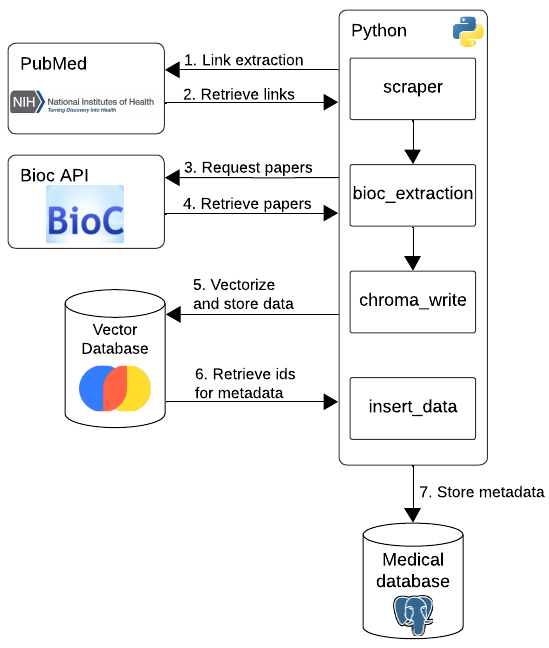
\includegraphics[width=0.75\textwidth]{images/ETL_Pipeline.png} %specify width
	\end{center}
	\caption{Medical Data Extraction Pipeline} %specify caption
	\label{fig:etl}
\end{figure}

\begin{multicols}{2}
	\begin{itemize}[topsep=0pt, partopsep=0pt, parsep=0pt]
	
	\item{allergy}
	\item{bird flu}
	\item{cancer}
	\item{chickenpox}
	\item{common cold}
	\item{conjunctivitis}
	\item{covid sickness}
	\item{covid symptoms}
	\item{covid treatment}
	\item{covid vaccine}
	\item{flu vaccine}
	\item{headache}
	\item{influenza}
	\item{monkeypox}
	\item{stomach aches}
	\item{swine flu}
	\item{zika}

	\end{itemize}

\end{multicols}



To extract them, we built a scraper in Python using Selenium and BeautifulSoup libraries. We used Selenium to retrieve the web source from PubMed's website, and BeautifulSoup was used to get the links to each paper. These links contained the PMC identifier. For each topic, we selected 5,000 PMC identifiers. These identifiers were grouped by topic and stored locally in Comma Separated Value (CSV) files.

\subsection{BioC API}
After retrieving those identifiers, we need to extract the research papers. Using the PubMed API, BioC, we made requests that returned the documents as JSON. These JSONs were preprocessed to contain texts, and we removed tables and figures. Later, the paper's sections -introduction, methodology, results, and others- were combined as one attribute, excluding references. We removed tables, figures, and references from the context to ensure the chunking process worked appropriately. If the data is not preprocessed, when performing RAG, we can retrieve data that is not useful. After that, we turned the result into a new JSON that contained the research metadata and its context. 

\subsection{Vectorizing data}
Later, each research paper’s context was split into chunks using LangChain. Then, we used an LLM, BAAI \cite{bge_embedding}, to embed these chunks. A universal unique identifier (UUID) was combined with each chunk and stored in a Chroma \cite{chroma} database. After uploading the data to Chroma, we added these UUIDs to their JSON. 


\subsection{Store metadata}
Now, with all papers vectorized, we upload the metadata into a Postgres database. First, we validate that there are no duplicate records in the system. To prevent duplicates, we search for the paper's reference. If any is found, we delete the chunks from the vector database. Additionally, any research that did not contain at least an abstract was removed. That ensures that there is no repetition or inconsistency when doing the rebuttal. Later, we upload this data into the system following the schema found in Figure \ref{fig:table}. The tables in this schema are as follow:

\begin{description}
	\item{\textbf{Research:}}  The table contains the research paper data. Its attributes are title, which is the research paper title; context, the paper’s text; paper\_ref, the complete reference of the paper, used to prevent duplicates; and fullpaper, which is a boolean that is true if the paper contains an abstract, introduction, methodology, discussion, conclusion, and references.
	\item{\textbf{Chunks:}} This table pairs the UUIDs from the paper's chunks and their respective research record.  
	\item{\textbf{Keyword:}} Some research papers contain keywords that allow the reader to know the subjects mentioned in the paper. 
	\item{\textbf{Author:}} Stores the first and last names of all authors identified in the research paper. 
	\item{\textbf{Reference:}} All references that are present in the research paper.
	\item{\textbf{Topic:}} This contains the different topics used to search the papers.

\end{description}

\begin{figure}[H]
	\begin{center}
		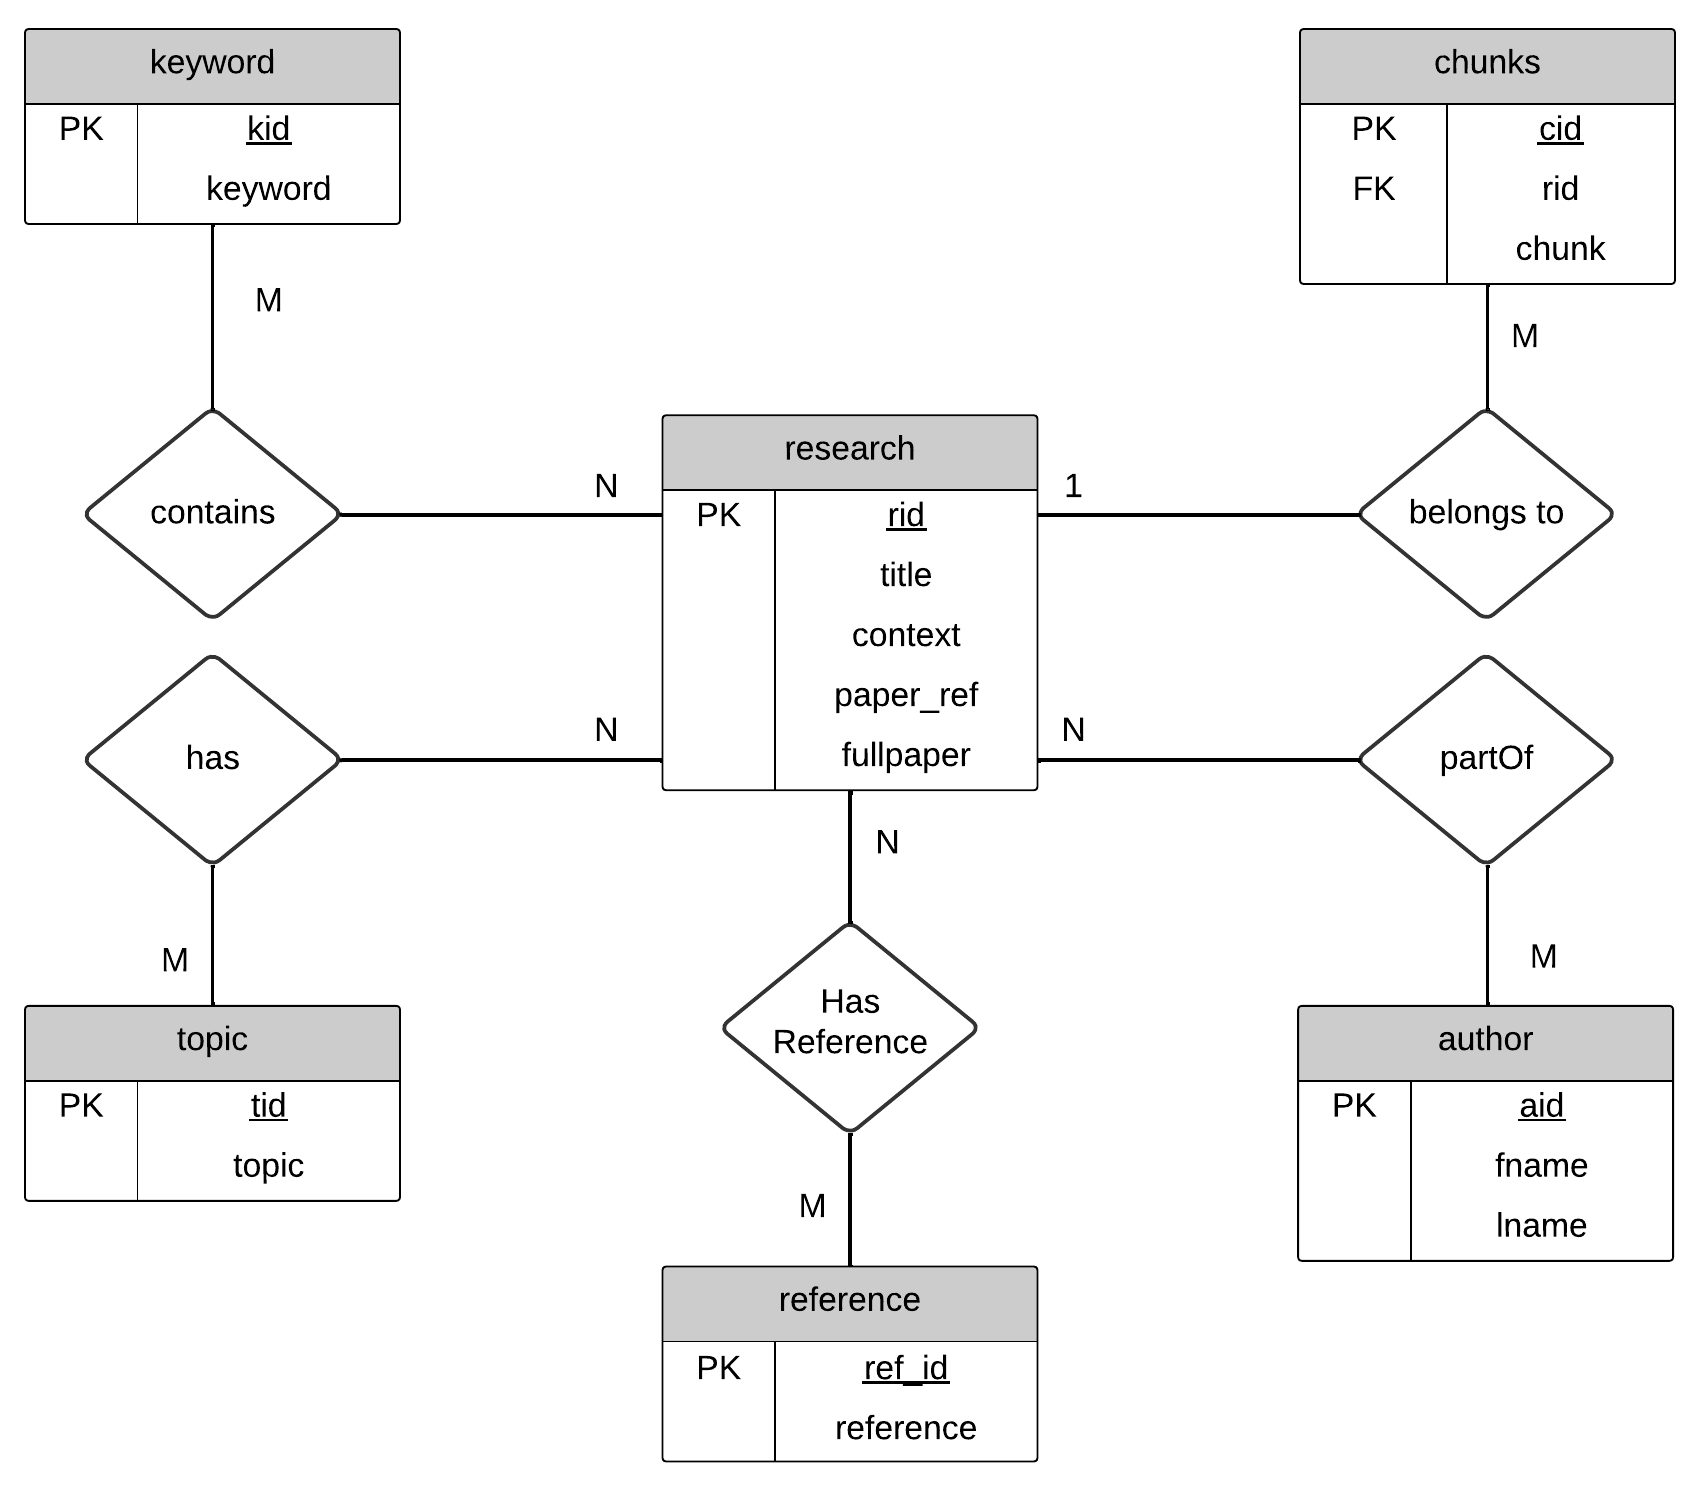
\includegraphics[width=0.9\textwidth]{images/Table_diagram.png} %specify width
	\end{center}
	\caption{Research Papers Schema Diagram} %specify caption
	\label{fig:table}
\end{figure}


We started the search with 85,000 peer-reviewed papers. After finishing the filtering and data cleaning, we ended with 56,365 different research papers. 



\section{Misinformation Rebuttal Pipeline}
After training the models and storing the context for the rebuttal, we create the model pipeline. The pipeline shown in Figure \ref{fig:llm} shows the process of receiving a text, making the classifications, and returning an explanation of why it is misinformation.

\begin{figure}[H]
	\begin{center}
		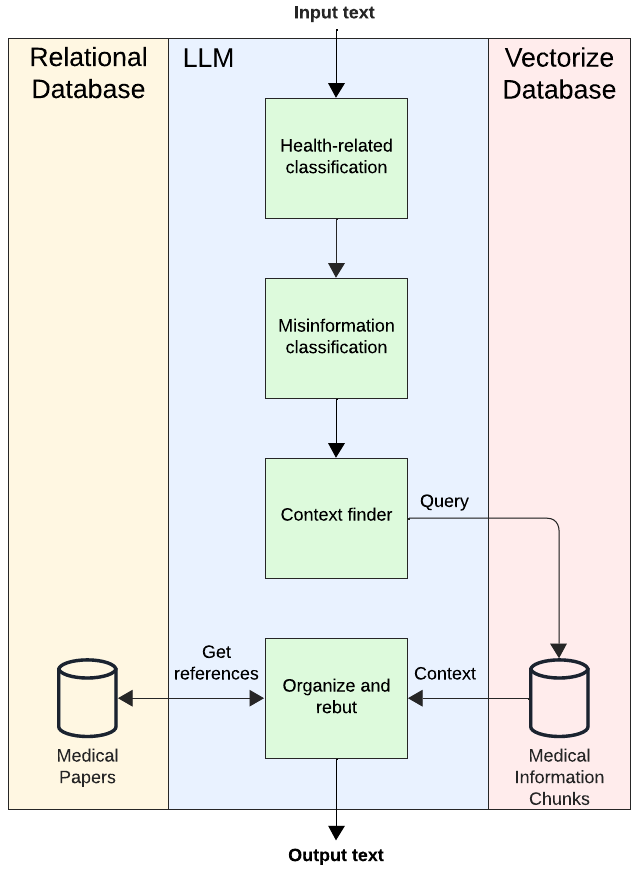
\includegraphics[width=0.75\textwidth]{images/LLM_Pipeline} %specify width
	\end{center}
	\caption{Misinformation Rebuttal LLM System Architecture} %specify caption
	\label{fig:llm}
\end{figure}


\subsection{Health-related Classification}
The first part of the pipeline is determining if the text is related to health. When the system receives the input text, it sends it to a model finetuned to classify health-related texts. This model determines whether the input is related, unrelated, or ambiguous.
If the text is health-related, we continue to the next part of the pipeline. When the text is non-related or ambiguous, we end the process. We end this because other topics are out of the model's scope. 

\subsection{Misinformation Classification}
After confirming that the text is health-related, we want to validate that it contains misinformation. The finetuned model can only return two possible results: misinformation or non-misinformation. If the model finds no misinformation after evaluating the text,
the final output will return both classifications. When the result contains misinformation, we start the search for research papers.

\subsection{Context Finder}
Before starting the search on the vector database, we must understand the topic of the text. To understand the text, we send a query to Ollama asking it to make a one-sentence query for the vector database related to the input.

 
 \begin{tcolorbox}[colback=gray!10, colframe=black!70, title=Input]
\texttt{%
\#nih fauci, @cdcdirector @sgottliebfda \&amp; @barda bright expected to be grilled tomorrow over ineffective \#flu vaccine at @housecommerce \#suboversight bets on fauci saying universal \#influenza vax in 5, maybe 10 years? my preview here: \url{https://t.co/fsqefwhik7} \#cdc \#fda \#vaccines%
}
\end{tcolorbox}

\begin{tcolorbox}[colback=white, colframe=black!70, title=Output]
\textit{%
Flu vaccine effectiveness and future universal influenza vaccination strategies.%
}
\end{tcolorbox}
 
The above example shows that Ollama can identify the topics of the original text. That tweet mentions that the flu vaccine is ineffective and asks how long it will take for a universal influenza vaccine. The LLM identified the topic and made a query that can help find
research papers related to it. However, it is essential to mention that the LLM output can vary. As mentioned previously, this is a statistical model and can have slight variations in its result. Now, this output is sent to the Chroma database to retrieve chunks of research
papers. For this experiment, our model returns eight chunks that are closest in context to the query. These chunks are then sent to another model to be analyzed and organized.

\subsection{Organize and Rebut}
The final part of our pipeline is using RAG to provide an answer that explains why the original text is misinformation. First, we retrieve the references of the chunks we use for the context. Then, we send the original text with the chunks, as context, to Ollama for
the model to evaluate. Ollama returns a 2-3 sentence result that explains the text’s misinformation. The final output is a JSON with the following attributes:

\begin{description}
\item{\textbf{chroma\_value:}} If the text is health-related and is misinformation, this will have the rebuttal output from Ollama, consisting of 2-3 sentences. If the text is non-related or non-misinformation, it will give a default value saying so. 
\item{\textbf{health:}} This is the input text health classification.
\item{\textbf{misinformation:}} This is the input text misinformation classification.
\item{\textbf{references:}} This attribute stores the list of references used for the rebuttal. 
\item{\textbf{t\_context:}} The original text.

\end{description}

The pipeline enables us to automate the classification process and rebut misinformation using peer-reviewed research. By leveraging fine-tuned models, vector search, and RAG, the architecture provides concise, fact-based responses. A key advantage of this
approach is its ability to explain complex content accessible to non-technical readers, giving them a clearer understanding of false information. This can assist professionals in the field to mitigate the spread of lies that can negatively impact public health.

%\begin{lstlisting}[language=json]
%{
%  "chroma_value": "The text claims that the current flu vaccine is ineffective and implies a specific timeline for developing a universal influenza vaccine. However, researchers are still working on overcoming the limitations of current influenza vaccines, ...",
%  "health": "Related",
%  "misinformation": "Misinformation",
%  "references": "[Choi A, Garcia-Sastre A, Schotsaert M. Host immune response-inspired development of the influenza vaccine.  2020;125:28-35. doi: 10.1016/j.anai.2020.04.008., ... ]",
%  "t_context": "#nih fauci, @cdcdirector @sgottliebfda &amp; @barda bright expected ...",
%}
%\end{lstlisting}



%\begin{enumerate}
	%\item Health-related classification: Verifies if the inputted text is health-related. The possible options are related, unrelated, or ambiguous.
	%\item Misinformation classification: If the text was classified as health-related, we then checks if the text contains misinformation. If any misinformation is detected, we need to find official health data to rebut said misinformation.
	%\item	Context finder: A query is created for a vector database based on the original text. This query is sent to a vectorized database, Chroma, and will return chunks that are related to the query.
	%\item	Medical information database:  This is a database that contains medical metadata from official sources. Using the chunk IDs we will retrieve the original papers' references.
	%\item	Organize and rebut: The result from the medical database is now processed and used to make a rebuttal for the misinformation in the text. Then, we query the relational database to extract the references of the papers used for the previous part.
	%The output includes the original text, the health and misinformation classifications, the correction of the misinformation, and the citation of the sources used. 
%\end{enumerate}









